% !TEX TS-program = pdflatex
% !TEX encoding = UTF-8 Unicode
\documentclass[a4paper,11pt,openright,BCOR=15mm]{scrbook}

\usepackage[onehalfspacing]{setspace}
\usepackage[utf8]{inputenc}
\usepackage[portuges,english]{babel}
\usepackage[square,numbers]{natbib}
\usepackage{graphicx}
\usepackage[pdftex]{hyperref}
\usepackage[T1]{fontenc}
\usepackage{pdfpages}
\usepackage{lettrine}
\usepackage{booktabs}
\usepackage{scrhack}
\usepackage{scrlayer-scrpage}
\usepackage{ulem}
\usepackage{xcolor}
\usepackage{float}
\usepackage{placeins}
\usepackage{array}
\usepackage{amsmath}
\usepackage{amssymb}
\definecolor{cinza1}{RGB}{200,200,200}
\definecolor{cinza2}{RGB}{70,70,70}
\usepackage{vhistory}
\usepackage{listings}
\usepackage{color}
\usepackage{subcaption}
\usepackage{multirow}

\definecolor{dkgreen}{rgb}{0,0.6,0}
\definecolor{gray}{rgb}{0.5,0.5,0.5}
\definecolor{mauve}{rgb}{0.58,0,0.82}

\lstset{frame=tb,
    language=Java,
    aboveskip=3mm,
    belowskip=3mm,
    showstringspaces=false,
    columns=flexible,
    basicstyle={\small\ttfamily},
    numbers=none,
    numberstyle=\tiny\color{gray},
    keywordstyle=\color{blue},
    commentstyle=\color{dkgreen},
    stringstyle=\color{mauve},
    breaklines=true,
    breakatwhitespace=true,
    tabsize=3,
    extendedchars=true,
    inputencoding=utf8
}

\newcommand\ChapterFont{}
\newcommand\SectionFont{}
\pagestyle{scrheadings}
\ifoot[]{\raisebox{-32pt}{
\includegraphics[width=0.15\textwidth]{logos/logoisep}}}
\ofoot[]{\raisebox{-22pt}{
\includegraphics[width=0.10\textwidth]{logos/logo_DEI_big_transparente}}}
\cfoot[\pagemark]{\pagemark}
\automark[section]{chapter}
\usepackage{blindtext}
\usepackage{listings}
\usepackage{fancyvrb}
\usepackage[mono=false]{libertine}

\begin{document}

\selectlanguage{portuguese}
\frontmatter

\titlehead{
\includegraphics[scale=0.2]{logos/logoisep}
\hfill 
\includegraphics[scale=0.115]{logos/logo_DEI_big_transparente}}

\title{Equalização de Histograma e Processamento Paralelo em Java}
\subtitle{Sistemas Multinúcleo e Distribuídos}

\author{Mestrado em Engenharia Informática -- 2025/2026}

\publishers{
    Luis Manuel Nazário Mendes Santos\\
    \texttt{Versão \vhCurrentVersion, \vhCurrentDate}\\
}

\date{Porto, maio de 2026}

\maketitle

\cleardoublepage

\tableofcontents
\addcontentsline{toc}{chapter}{Lista de Figuras}
\listoffigures
\addcontentsline{toc}{chapter}{Lista de Tabelas}
\listoftables

\chapter*{Declaração de Integridade}
\addcontentsline{toc}{chapter}{Declaração de Integridade}

Declaro, por este meio, que o presente trabalho académico foi realizado com integridade.\newline

Afirmo não ter recorrido a plágio, falsificação de resultados ou qualquer outra forma de utilização indevida de informação no decurso da sua elaboração.\newline

Assim, o trabalho aqui apresentado é original e da minha autoria, não tendo sido previamente utilizado para outros fins que não os explicitamente reconhecidos. Este documento identifica de forma transparente o modo como foram utilizadas ferramentas de IA, bem como o propósito dessa utilização.\newline

Confirmo ainda o meu conhecimento e respeito pelo Código de Conduta Ética do P.PORTO.\newline

ISEP, Porto, 11 de maio de 2026

\mainmatter

% ============================================================
\chapter{Introdução}
% ============================================================

O processamento digital de imagem é uma área com aplicações em medicina, fotografia, visão por computador e muitas outras disciplinas. Uma das operações mais fundamentais é a \textbf{equalização de histograma}, que redistribui as intensidades dos píxeis de modo a aumentar o contraste de imagens de baixo contraste.

Neste projeto, implementa-se a equalização de histograma em Java, explorando diferentes estratégias de concorrência: solução sequencial, multithreading manual, thread pools, o framework Fork/Join e o paradigma assíncrono com \texttt{CompletableFuture}. O objetivo não é apenas a correção dos resultados, mas também a análise de desempenho e escalabilidade de cada abordagem.

\begin{figure}[H]
    \centering
    \begin{subfigure}[b]{0.45\textwidth}
        \centering
        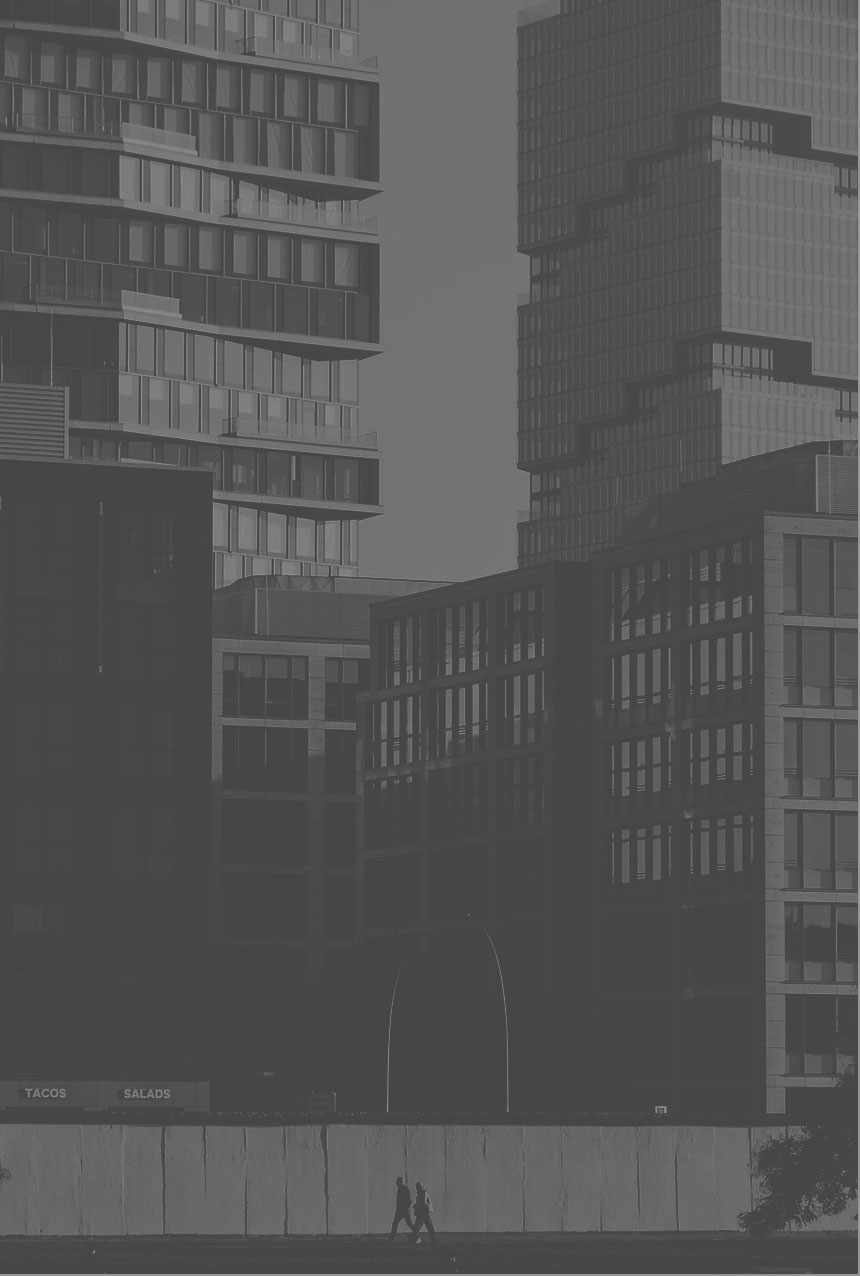
\includegraphics[width=\textwidth]{../../images/in/src.jpg}
        \caption{Imagem original}
    \end{subfigure}
    \hfill
    \begin{subfigure}[b]{0.45\textwidth}
        \centering
        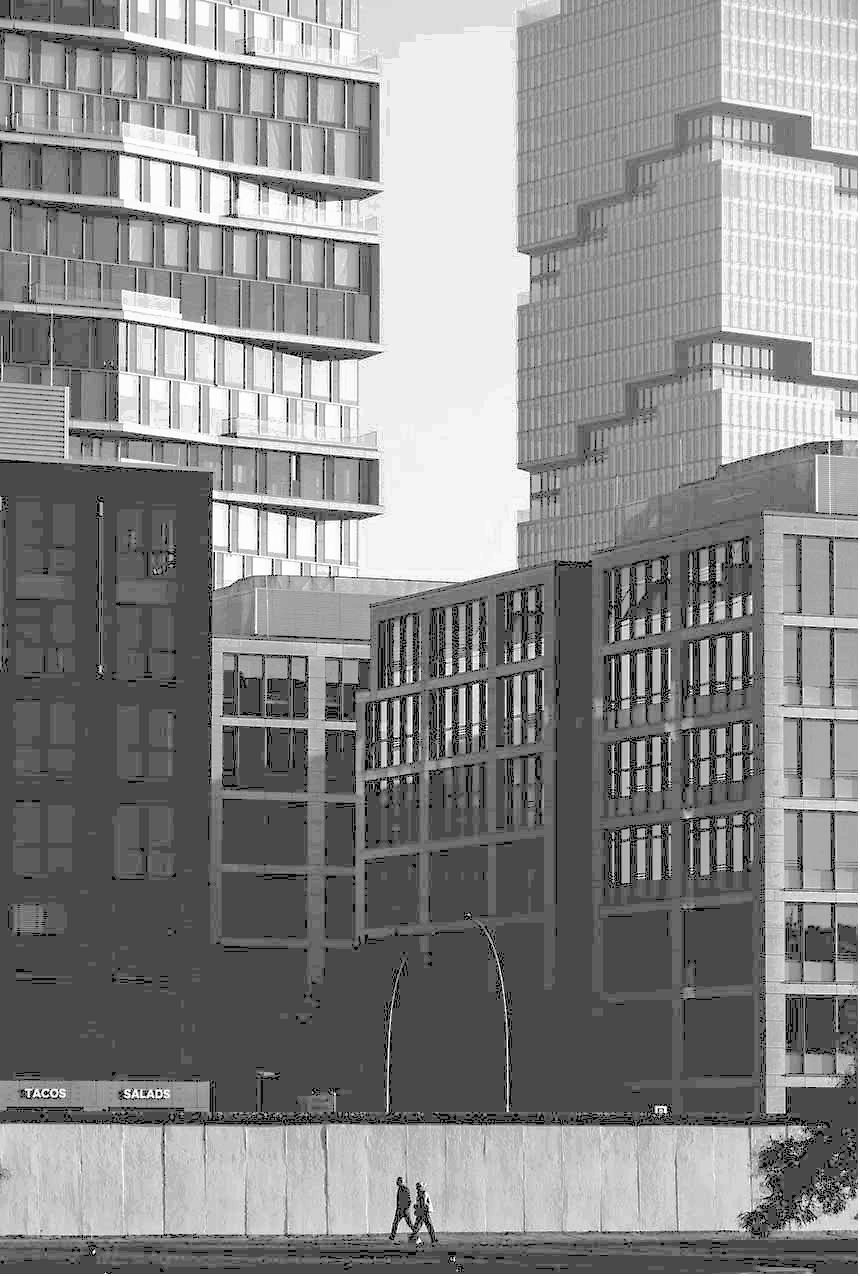
\includegraphics[width=\textwidth]{../../images/out/src_sequential.jpg}
        \caption{Imagem após equalização sequencial}
    \end{subfigure}
    \caption{Efeito visual da equalização de histograma (imagem 860×1276)}
    \label{fig:before_after}
\end{figure}

Os testes foram executados numa máquina com \textbf{22 processadores lógicos}. O conjunto de imagens de teste cobre quatro dimensões distintas para análise de escalabilidade: 512×512 (262~144 px), 860×1276 (1~097~360 px), 1920×1080 (2~073~600 px) e 3840×2160 (8~294~400 px).

O algoritmo de equalização é dividido em três fases:
\begin{enumerate}
    \item \textbf{Histograma de luminosidade:} array de 256 inteiros onde a posição $i$ contém o número de píxeis com luminosidade $i$.
    \item \textbf{Histograma cumulativo:} array de 256 inteiros onde a posição $i$ contém o número de píxeis com luminosidade $\leq i$.
    \item \textbf{Reescrita dos píxeis:} cada píxel é transformado segundo:
    \[
        \text{newLuminosity} = \left\lfloor 255 \times \frac{\text{cumulativeHist}[L]}{\text{totalPixels}} \right\rfloor
    \]
\end{enumerate}

% ============================================================
\chapter{Objetivos}
% ============================================================

O projeto tem como objetivos principais:

\begin{itemize}
    \item Implementar a equalização de histograma com diferentes abordagens de concorrência em Java.
    \item Comparar o desempenho (tempo de execução, consumo de memória, escalabilidade) de cada implementação.
    \item Explorar mecanismos de sincronização e garantir \textit{thread safety} em todas as implementações paralelas.
    \item Configurar e analisar o impacto de diferentes \textit{Garbage Collectors} da JVM no desempenho da aplicação.
    \item Documentar e justificar as escolhas de design e concorrência em cada abordagem.
\end{itemize}

A estrutura do projeto foi organizada em pacotes Java de acordo com a responsabilidade de cada componente:

\begin{itemize}
    \item \texttt{sismd.filters} --- Interface, classe base e todas as implementações do filtro.
    \item \texttt{sismd.benchmark} --- Infraestrutura de medição de desempenho.
    \item \texttt{sismd.utils} --- Utilitários de I/O de imagem (código fornecido pelo docente).
    \item \texttt{sismd.starter} --- Código de demonstração original fornecido pelo docente.
    \item \texttt{sismd.Main} --- Ponto de entrada com menu interativo.
\end{itemize}

% ============================================================
\chapter{Implementações}
% ============================================================

Todas as implementações partilham uma interface comum \texttt{HistogramEqualizer} e estendem a classe abstrata \texttt{AbstractFilter}, que disponibiliza os métodos utilitários \texttt{computeLuminosity}, \texttt{buildCumulativeHistogram} e \texttt{equalizedLuminosity}. Os métodos \texttt{computeHistogram} e \texttt{applyEqualization} da \texttt{SequentialFilter} têm visibilidade de pacote (\textit{package-private}) e são reutilizados pelas implementações paralelas como operações de folha.

% ============================================================
\section{Solução Sequencial}
% ============================================================

A solução sequencial serve como linha de base (\textit{baseline}) para comparação de desempenho. Processa o array de píxeis em três passagens sequenciais correspondentes às três fases do algoritmo.

\textbf{Justificação:} A implementação sequencial não tem overhead de criação de threads nem de sincronização, pelo que representa o custo mínimo do algoritmo. É indispensável para calcular o \textit{speedup} das implementações paralelas e para verificar a correção dos resultados.

\begin{lstlisting}[caption={Núcleo da implementação sequencial}]
public Color[][] apply(Color[][] image) {
    Color[][] result = Utils.copyImage(image);
    int totalPixels = result.length * result[0].length;

    int[] hist       = computeHistogram(result, 0, result.length);
    int[] cumulative = buildCumulativeHistogram(hist);
    applyEqualization(result, 0, result.length, cumulative, totalPixels);

    return result;
}
\end{lstlisting}

% ============================================================
\section{Multithreaded sem Thread Pool}
% ============================================================

Esta implementação cria e gere threads manualmente, sem reutilização. A estratégia divide as linhas da imagem igualmente entre as threads disponíveis.

\textbf{Estratégia de concorrência:}
\begin{enumerate}
    \item \textbf{Fase 1 (paralela):} Cada thread calcula um histograma parcial para as suas linhas, sem qualquer sincronização --- não há estado partilhado durante esta fase.
    \item \textbf{Barreira:} A thread principal aguarda a conclusão de todas as threads com \texttt{join()} e faz o merge dos histogramas parciais (256 iterações, custo desprezável).
    \item \textbf{Fase 2 (sequencial):} O histograma cumulativo é calculado sequencialmente (O(256)).
    \item \textbf{Fase 3 (paralela):} Cada thread reescreve os seus píxeis --- as threads acedem a linhas disjuntas, pelo que não há necessidade de sincronização.
\end{enumerate}

\textbf{Justificação:} A ausência de \textit{locks} ou variáveis atómicas durante as fases paralelas elimina o overhead de sincronização. A opção por histogramas parciais por thread (em vez de um array partilhado com \texttt{AtomicIntegerArray}) evita falsa partilha de cache e contention.

\begin{lstlisting}[caption={Fase paralela de histograma com threads manuais}]
for (int t = 0; t < actualThreads; t++) {
    final int id    = t;
    final int start = id * rows / actualThreads;
    final int end   = (id + 1) * rows / actualThreads;
    threads[t] = new Thread(() ->
        partialHists[id] = SequentialFilter.computeHistogram(result, start, end)
    );
    threads[t].start();
}
joinAll(threads); // barreira: aguarda todas as threads

int[] hist = new int[256];
for (int[] partial : partialHists)
    for (int i = 0; i < 256; i++) hist[i] += partial[i];
\end{lstlisting}

% ============================================================
\section{Thread Pool com ExecutorService}
% ============================================================

Esta implementação substitui a criação manual de threads por um pool fixo gerido pelo \texttt{ExecutorService}. As threads são reutilizadas entre as fases 1 e 3, eliminando o custo de criação e destruição de threads.

\textbf{Justificação:} Em cenários com muitas execuções do filtro (como o benchmark), o overhead de criar e destruir threads a cada execução pode ser significativo. O thread pool amortiza esse custo. As tarefas de histograma retornam \texttt{Future<int[]>}, permitindo recolher os resultados de forma limpa sem variáveis partilhadas.

\begin{lstlisting}[caption={Submissão de tarefas ao thread pool}]
List<Future<int[]>> histFutures = new ArrayList<>(actualThreads);
for (int t = 0; t < actualThreads; t++) {
    final int start = t * rows / actualThreads;
    final int end   = (t + 1) * rows / actualThreads;
    histFutures.add(pool.submit(() ->
        SequentialFilter.computeHistogram(result, start, end)
    ));
}
int[] hist = new int[256];
for (Future<int[]> f : histFutures) {
    int[] partial = f.get();
    for (int i = 0; i < 256; i++) hist[i] += partial[i]; 
}
\end{lstlisting}

% ============================================================
\section{Fork/Join Framework}
% ============================================================

A implementação Fork/Join utiliza o paradigma de \textit{divide-and-conquer} para dividir recursivamente o array de linhas até atingir um limiar (\texttt{THRESHOLD = 32} linhas), a partir do qual a computação é sequencial.

\textbf{Estratégia:}
\begin{itemize}
    \item \texttt{HistogramTask} (\texttt{RecursiveTask<int[]>}): divide o intervalo de linhas ao meio; a metade esquerda é bifurcada (\texttt{fork}), a metade direita é computada na thread atual (\texttt{compute}), e depois faz-se \texttt{join} + merge.
    \item \texttt{EqualizationTask} (\texttt{RecursiveAction}): usa \texttt{invokeAll} para executar ambas as metades em paralelo.
\end{itemize}

\textbf{Justificação:} O \texttt{ForkJoinPool} usa \textit{work stealing}: threads que ficam sem tarefas roubam tarefas de outras, maximizando a utilização dos processadores. O limiar de 32 linhas foi escolhido de modo a criar tarefas granulares suficientes para manter todas as threads ocupadas sem excessivo overhead de \textit{forking}.

\begin{lstlisting}[caption={HistogramTask com Fork/Join}]
@Override
protected int[] compute() {
    if (end - start <= THRESHOLD)
        return SequentialFilter.computeHistogram(image, start, end);

    int mid = (start + end) >>> 1;
    HistogramTask left  = new HistogramTask(image, start, mid);
    HistogramTask right = new HistogramTask(image, mid, end);

    left.fork();                      // execucao assincrona
    int[] rightResult = right.compute();  // execucao sincrona
    int[] leftResult  = left.join();      // aguarda left

    for (int i = 0; i < 256; i++) leftResult[i] += rightResult[i];
    return leftResult;
}
\end{lstlisting}

% ============================================================
\section{CompletableFuture}
% ============================================================

A implementação com \texttt{CompletableFuture} usa programação assíncrona declarativa para expressar a composição de tarefas sem gestão explícita de threads ou bloqueios.

\textbf{Estratégia:}
\begin{itemize}
    \item \texttt{supplyAsync} lança as tarefas de histograma assincronamente num \texttt{ExecutorService} dedicado.
    \item \texttt{CompletableFuture.allOf(...).thenApply(...)} aguarda a conclusão de todas as tarefas e executa o merge como uma continuação não bloqueante.
    \item \texttt{runAsync} lança as tarefas de equalização; \texttt{allOf(...).join()} aguarda a conclusão.
\end{itemize}

\textbf{Justificação:} O \texttt{CompletableFuture} permite expressar dependências entre tarefas de forma declarativa. O uso de \texttt{thenApply} para o merge garante que este só ocorre após todas as tarefas estarem completas, sem \textit{polling} nem bloqueio prematuro. O \texttt{join()} sobre os futuros dentro do \texttt{thenApply} é não bloqueante porque todos já terminaram no momento em que \texttt{allOf} dispara a continuação.

\begin{lstlisting}[caption={Merge assíncrono com allOf e thenApply}]
int[] hist = CompletableFuture
    .allOf(histFutures.toArray(new CompletableFuture[0]))
    .thenApply(v -> {
        int[] merged = new int[256];
        for (CompletableFuture<int[]> f : histFutures) {
            int[] partial = f.join(); // nao bloqueia: todos ja concluiram
            for (int i = 0; i < 256; i++) merged[i] += partial[i];
        }
        return merged;
    })
    .join();
\end{lstlisting}

% ============================================================
\section{Tuning do Garbage Collector}
\label{sec:gc}
% ============================================================

O benchmark foi executado separadamente com quatro \textit{Garbage Collectors} da JVM (\texttt{-Xms256m -Xmx2g}), usando a imagem 1920×1080 como referência. Os logs de pausas foram capturados com \texttt{-Xlog:gc:<ficheiro>.log}.

\subsection{Garbage Collectors Avaliados}

\textbf{Serial GC} (\texttt{-XX:+UseSerialGC}): Usa uma única thread de GC, com pausas \textit{stop-the-world} longas (média 32~ms, máx. 69~ms). Surpreendentemente, produz o \textbf{menor tempo de execução} neste benchmark (43~ms sequencial, 8~ms melhor paralelo) porque não tem threads concorrentes a competir com a aplicação nem \textit{write barriers} complexas.

\textbf{Parallel GC} (\texttt{-XX:+UseParallelGC}): Múltiplas threads de GC reduzem a pausa média para 12.6~ms (máx. 40.9~ms). Tempo de execução comparável ao Serial GC (41~ms sequencial). Optimizado para throughput, à custa de maior variância nas pausas.

\textbf{G1GC} (\texttt{-XX:+UseG1GC}): Divide a heap em regiões e recolhe as mais rentáveis primeiro. Pausas curtas e previsíveis (média 7.9~ms, máx. 10.8~ms). Contudo, o overhead da gestão de regiões e das \textit{write barriers} aumenta o tempo sequencial para 62~ms (+44\% face ao Serial GC).

\textbf{ZGC} (\texttt{-XX:+UseZGC}): Recolha maioritariamente concorrente — sem pausas \textit{stop-the-world} significativas. No entanto, os threads de marcação concorrentes disputam os 22 núcleos com a aplicação, elevando o tempo sequencial para 71~ms (+65\% face ao Serial GC) e a memória consumida para ~112--132~MB.

\subsection{Resultados}

\begin{table}[H]
    \centering
    \caption{Comparação de GCs — imagem 1920×1080 (\texttt{-Xms256m -Xmx2g})}
    \label{tab:gc_comparison}
    \begin{tabular}{lrrrrrr}
        \toprule
        \textbf{GC} & \textbf{Seq. (ms)} & \textbf{Melhor (ms)} & \textbf{Speedup máx.} & \textbf{Eventos GC} & \textbf{Pausa média} & \textbf{Pausa máx.} \\
        \midrule
        Serial GC   & \textbf{43} &  \textbf{8} & \textbf{5.38×} & 121 & 32.0~ms & 69.1~ms \\
        Parallel GC &          41 &          10 &          4.10× & 176 & 12.6~ms & 40.9~ms \\
        G1GC        &          62 &          24 &          2.58× & 105 &  7.9~ms & 10.8~ms \\
        ZGC         &          71 &          26 &          2.73× & $\approx$0 & $\approx$0~ms & $\approx$0~ms \\
        \bottomrule
    \end{tabular}
\end{table}

As Figuras~\ref{fig:gc_timing} e~\ref{fig:gc_pauses} ilustram graficamente os dados acima.

\begin{figure}[H]
    \centering
    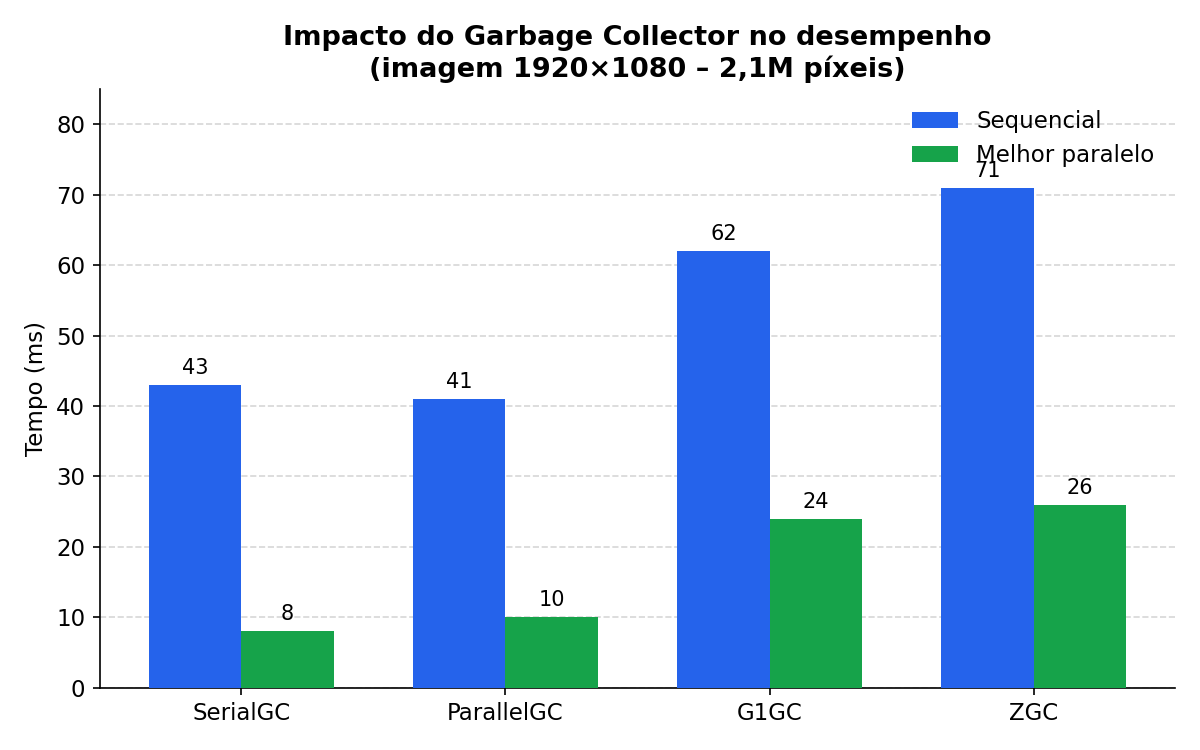
\includegraphics[width=0.82\textwidth]{../../images/charts/chart_04_gc_timing.png}
    \caption{Tempo sequencial e melhor paralelo por Garbage Collector}
    \label{fig:gc_timing}
\end{figure}

\begin{figure}[H]
    \centering
    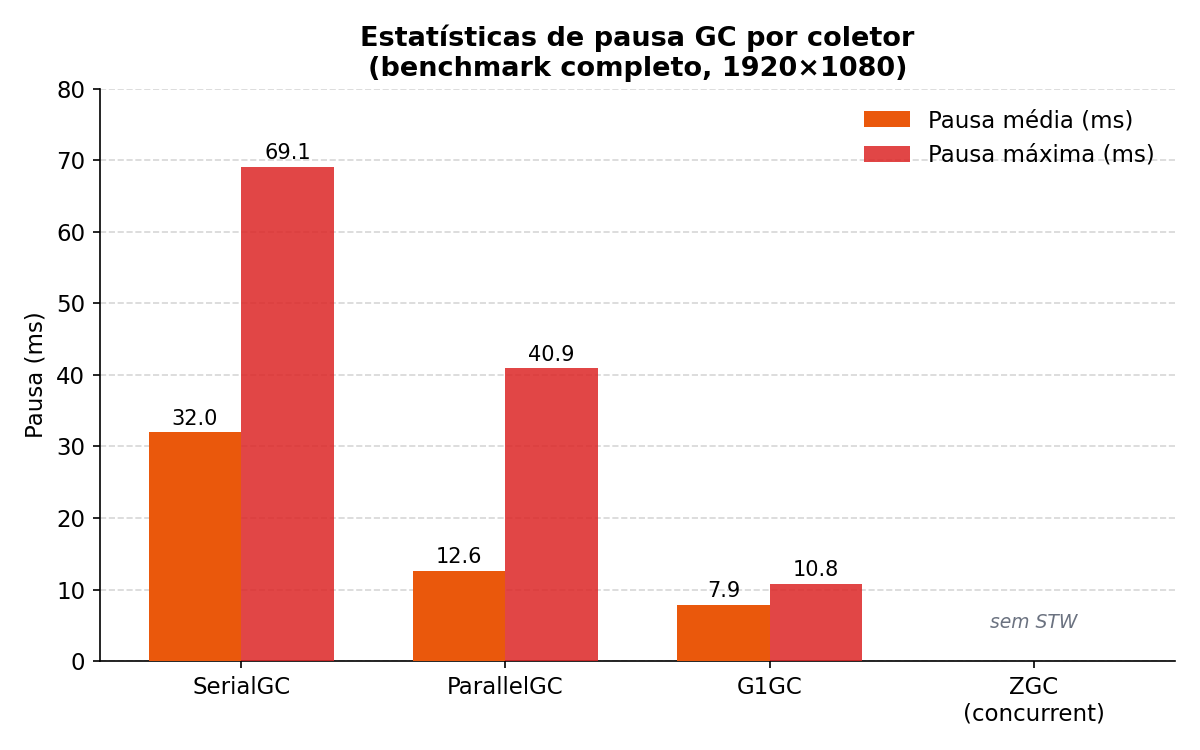
\includegraphics[width=0.82\textwidth]{../../images/charts/chart_05_gc_pauses.png}
    \caption{Estatísticas de pausa GC por coletor (benchmark completo)}
    \label{fig:gc_pauses}
\end{figure}

\subsection{Análise e Escolha}

O resultado mais contraintuitivo é que o \textbf{SerialGC produz o melhor throughput} apesar de ter as pausas mais longas. A razão é que as pausas ocorrem \emph{entre} medições (no \texttt{rt.gc()} explícito do benchmark), enquanto o que afeta o tempo medido é o overhead do GC durante a execução do filtro: \textit{write barriers}, alocação de regiões e threads de fundo concorrentes. O Serial GC não tem nenhum destes.

O \textbf{ZGC} é o polo oposto: zero pausas STW, mas threads de marcação concorrentes que disputam os 22 núcleos com a aplicação --- um custo desproporcionado para uma carga de trabalho \textit{compute-heavy} e de curta duração.

\textbf{Recomendação:}
\begin{itemize}
    \item \textbf{Processamento batch (máximo throughput):} Serial GC ou Parallel GC.
    \item \textbf{Serviço interativo (latência previsível):} G1GC com \texttt{-XX:MaxGCPauseMillis=100}.
    \item \textbf{Serviço de baixa latência com heap grande:} ZGC (não adequado para este workload).
\end{itemize}

Para este projeto, adota-se \textbf{G1GC} como configuração de referência por ser o padrão do JDK moderno e oferecer pausas previsíveis aceitáveis para uso interativo:
\begin{Verbatim}
-XX:+UseG1GC -XX:MaxGCPauseMillis=200
-XX:G1HeapRegionSize=4m -Xms256m -Xmx2g
\end{Verbatim}

% ============================================================
\chapter{Concorrência e Sincronização}
% ============================================================

\section{Estrutura das Fases}

O algoritmo de equalização de histograma tem uma estrutura de fases (\textit{pipeline barrier}):

\begin{enumerate}
    \item \textbf{Fase 1} (paralelizável): Computação do histograma — os píxeis são independentes.
    \item \textbf{Barreira}: Merge dos histogramas parciais — necessita que todas as threads da fase 1 tenham terminado.
    \item \textbf{Fase 2} (sequencial): O histograma cumulativo é calculado em O(256) --- custo negligenciável.
    \item \textbf{Fase 3} (paralelizável): Reescrita dos píxeis — independentes e em linhas disjuntas.
\end{enumerate}

\section{Thread Safety}

\textbf{Fase 1 (histograma):} Cada thread opera sobre um array local \texttt{int[256]}. Não há estado partilhado mutável. Após \texttt{join()}/\texttt{Future.get()}/\texttt{allOf().join()}, as escritas de todas as threads são visíveis na thread principal (garantia de \textit{happens-before} da API de concorrência Java).

\textbf{Merge:} Executado exclusivamente na thread principal. Não requer sincronização.

\textbf{Fase 3 (equalização):} Cada thread escreve em linhas disjuntas do array \texttt{result}. O array \texttt{cumulative} é lido mas nunca escrito pelas threads, pelo que não há \textit{data races}.

\section{Estruturas de Dados e Mecanismos}

\begin{table}[H]
    \centering
    \caption{Mecanismos de sincronização por implementação}
    \label{tab:sync}
    \begin{tabular}{lll}
        \toprule
        \textbf{Implementação} & \textbf{Sincronização} & \textbf{Justificação} \\
        \midrule
        Multithreaded  & \texttt{Thread.join()} & Barreira explícita entre fases \\
        Thread Pool    & \texttt{Future.get()}  & Bloqueante por tarefa; recolhe resultado \\
        Fork/Join      & \texttt{fork/join}, \texttt{invokeAll} & Implícito no framework \\
        CompletableFuture & \texttt{allOf().join()} & Composição declarativa de dependências \\
        \bottomrule
    \end{tabular}
\end{table}

A opção por histogramas parciais por thread (sem \texttt{synchronized} nem \texttt{AtomicIntegerArray}) é intencional: elimina \textit{contention} e falsa partilha de cache. O custo do merge (256 adições) é desprezável face ao trabalho paralelo.

% ============================================================
\chapter{Análise de Performance}
% ============================================================

\section{Configuração do Ambiente}

\begin{itemize}
    \item \textbf{JVM:} Java 21, sem flag explícita de GC (secção~\ref{sec:gc})
    \item \textbf{Imagens de teste:} 512×512, 860×1276, 1920×1080, 3840×2160
    \item \textbf{Processadores:} 22 lógicos (\texttt{Runtime.getRuntime().availableProcessors()})
    \item \textbf{Threads testadas:} 1, 2, 4, 8, 22
    \item \textbf{Metodologia:} 3 execuções de aquecimento (JIT) + média de 5 medições com \texttt{System.nanoTime()}
\end{itemize}

% ─────────────────────────────────────────────────────────────
\section{Resultados Globais (imagem 860×1276)}
% ─────────────────────────────────────────────────────────────

\begin{table}[H]
    \centering
    \caption{Benchmark completo — imagem 860×1276 (1~097~360 píxeis)}
    \label{tab:benchmark}
    \begin{tabular}{lrrr}
        \toprule
        \textbf{Implementação} & \textbf{Tempo (ms)} & \textbf{Memória (MB)} & \textbf{Speedup} \\
        \midrule
        Sequential                      & 33 & 40.29 & 1.00× \\
        \midrule
        Multithreaded -- 1 thread       & 24 & 39.92 & 1.38× \\
        Multithreaded -- 2 threads      & 16 & 40.32 & 2.06× \\
        Multithreaded -- 4 threads      &  9 & 40.36 & 3.67× \\
        Multithreaded -- 8 threads      &  6 & 42.00 & \textbf{5.50×} \\
        Multithreaded -- 22 threads     &  7 & 54.05 & 4.71× \\
        \midrule
        Thread Pool -- 1 thread         & 24 & 38.04 & 1.38× \\
        Thread Pool -- 2 threads        & 14 & 38.50 & 2.36× \\
        Thread Pool -- 4 threads        &  9 & 39.65 & 3.67× \\
        Thread Pool -- 8 threads        &  9 & 39.44 & 3.67× \\
        Thread Pool -- 22 threads       &  7 & 40.01 & 4.71× \\
        \midrule
        Fork/Join                       &  7 & 39.30 & 4.71× \\
        \midrule
        CompletableFuture -- 1 thread   & 23 & 38.04 & 1.43× \\
        CompletableFuture -- 2 threads  & 14 & 38.76 & 2.36× \\
        CompletableFuture -- 4 threads  & 10 & 39.77 & 3.30× \\
        CompletableFuture -- 8 threads  &  7 & 39.12 & 4.71× \\
        CompletableFuture -- 22 threads &  6 & 40.02 & \textbf{5.50×} \\
        \bottomrule
    \end{tabular}
\end{table}

O melhor speedup obtido é de \textbf{5.50×} (Multithreaded 8T e CompletableFuture 22T), partindo de 33~ms sequenciais até 6~ms. A Figura~\ref{fig:speedup_threads} ilustra a evolução do speedup com o número de threads para as três implementações paralelizáveis.

\begin{figure}[H]
    \centering
    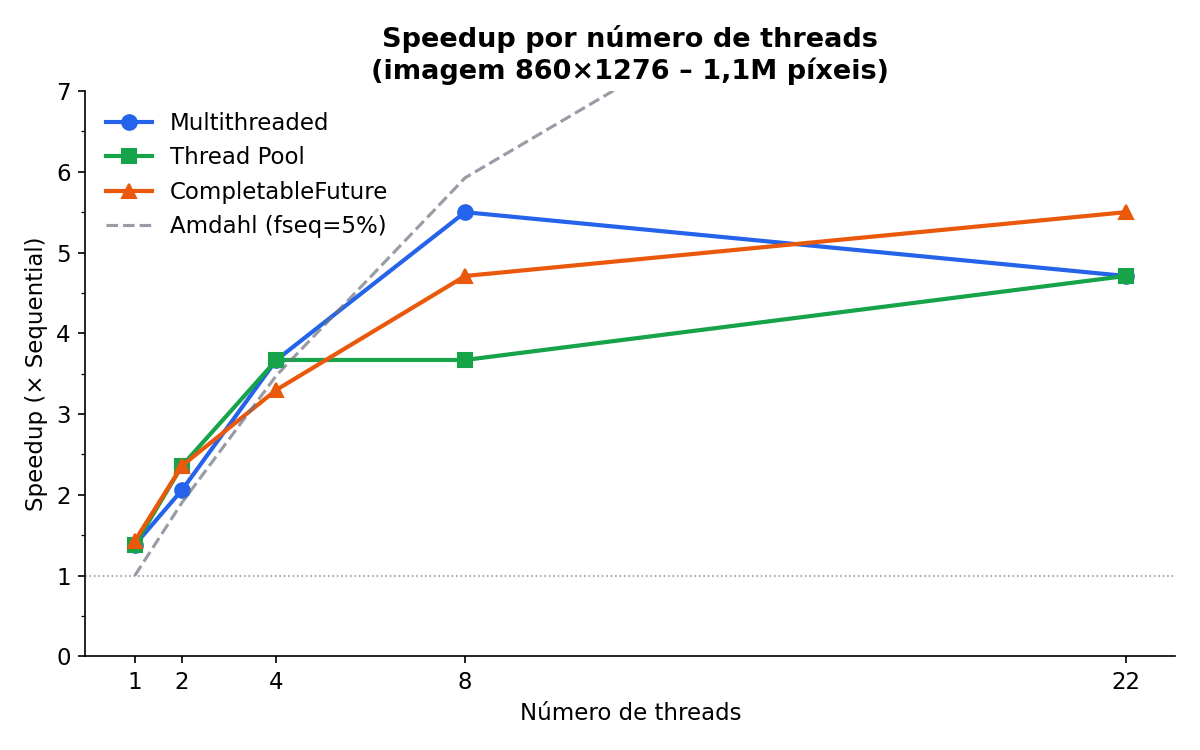
\includegraphics[width=0.85\textwidth]{../../images/charts/chart_01_speedup_threads.png}
    \caption{Speedup por número de threads (imagem 860×1276)}
    \label{fig:speedup_threads}
\end{figure}

Nota-se que o Multithreaded sem pool atinge o pico em 8 threads e regride ligeiramente para 22, enquanto o CompletableFuture continua a ganhar até 22 threads, evidenciando que o overhead de gestão do pool de tarefas é amortizado de forma diferente em cada abstração.

% ─────────────────────────────────────────────────────────────
\section{Escalabilidade por Dimensão de Imagem}
% ─────────────────────────────────────────────────────────────

A Figura~\ref{fig:time_by_size} mostra que o tempo sequencial cresce aproximadamente de forma linear com o número de píxeis --- o que é esperado, pois o algoritmo é O(N).

\begin{figure}[H]
    \centering
    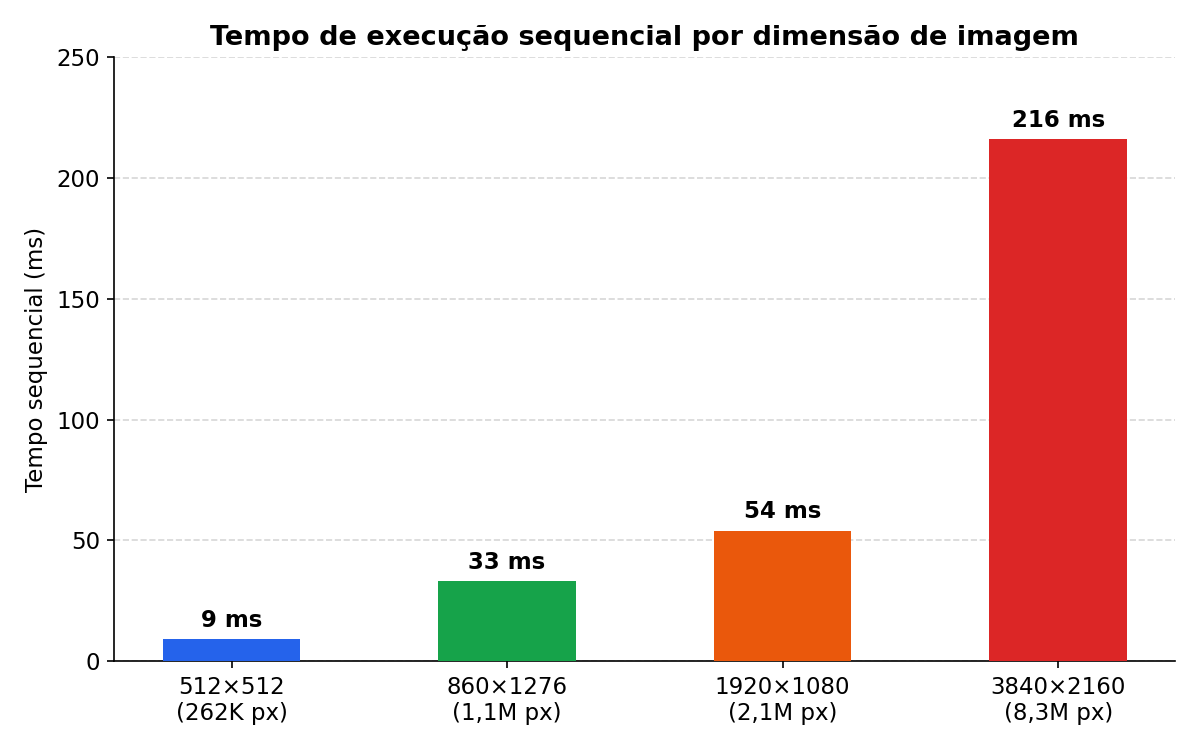
\includegraphics[width=0.80\textwidth]{../../images/charts/chart_02_time_by_size.png}
    \caption{Tempo sequencial em função da dimensão da imagem}
    \label{fig:time_by_size}
\end{figure}

\begin{table}[H]
    \centering
    \caption{Escalabilidade: tempo sequencial e melhor speedup por dimensão}
    \label{tab:scalability_size}
    \begin{tabular}{lrrrr}
        \toprule
        \textbf{Imagem} & \textbf{Píxeis} & \textbf{Seq. (ms)} & \textbf{Melhor (ms)} & \textbf{Speedup máx.} \\
        \midrule
        512×512      &    262~144 &   9 &  3 & 3.00× (TP/CF 8T) \\
        860×1276     &  1~097~360 &  33 &  6 & 5.50× (MT 8T, CF 22T) \\
        1920×1080    &  2~073~600 &  54 & 18 & 3.00× (MT 22T) \\
        3840×2160    &  8~294~400 & 216 & 79 & 2.73× (TP 22T) \\
        \bottomrule
    \end{tabular}
\end{table}

A Figura~\ref{fig:speedup_by_size} compara o melhor speedup de cada implementação para as quatro dimensões:

\begin{figure}[H]
    \centering
    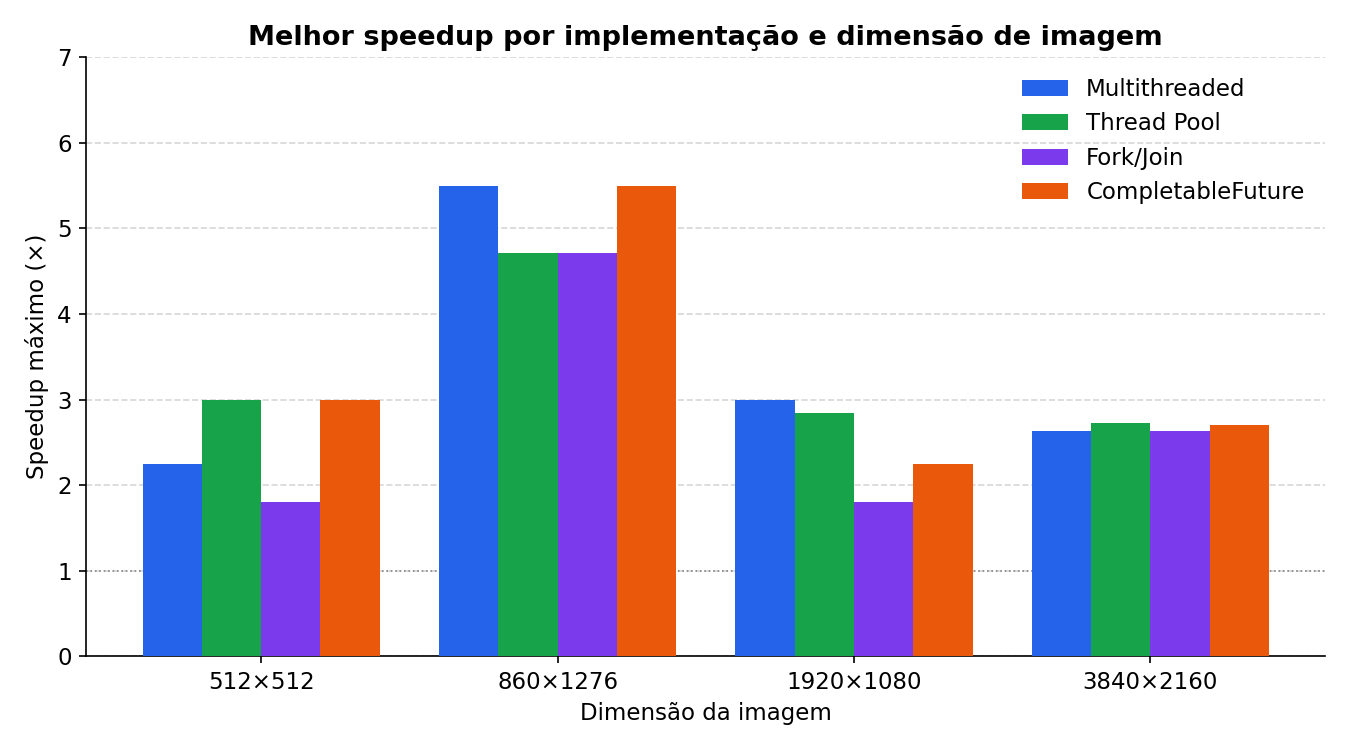
\includegraphics[width=0.90\textwidth]{../../images/charts/chart_03_speedup_by_size.png}
    \caption{Melhor speedup por implementação e dimensão de imagem}
    \label{fig:speedup_by_size}
\end{figure}

Observa-se um padrão não-monotónico: o speedup \textbf{cresce} da imagem pequena para a média (512→860×1276), mas \textbf{decresce} para as imagens grandes. Isto explica-se por dois fenómenos opostos:

\begin{itemize}
    \item \textbf{Imagens pequenas (512×512):} o overhead de threading é comparável ao trabalho útil --- o speedup máximo é apenas 3× apesar de 8 threads disponíveis.
    \item \textbf{Sweet spot (~1M píxeis):} o trabalho por thread é suficiente para amortizar os overheads; Multithreaded 8T e CF 22T atingem \textbf{5.50×}.
    \item \textbf{Imagens grandes (4K, 8.3M px):} todas as implementações a 22 threads convergem para ~79--82~ms. O bottleneck desloca-se da CPU para a \textbf{largura de banda de memória} --- a Lei de Amdahl aplicada a recursos de hardware, não apenas ao código.
\end{itemize}

A Figura~\ref{fig:time_threads_fhd} detalha o comportamento para Full~HD (2.1M píxeis), onde o Fork/Join degrada visivelmente:

\begin{figure}[H]
    \centering
    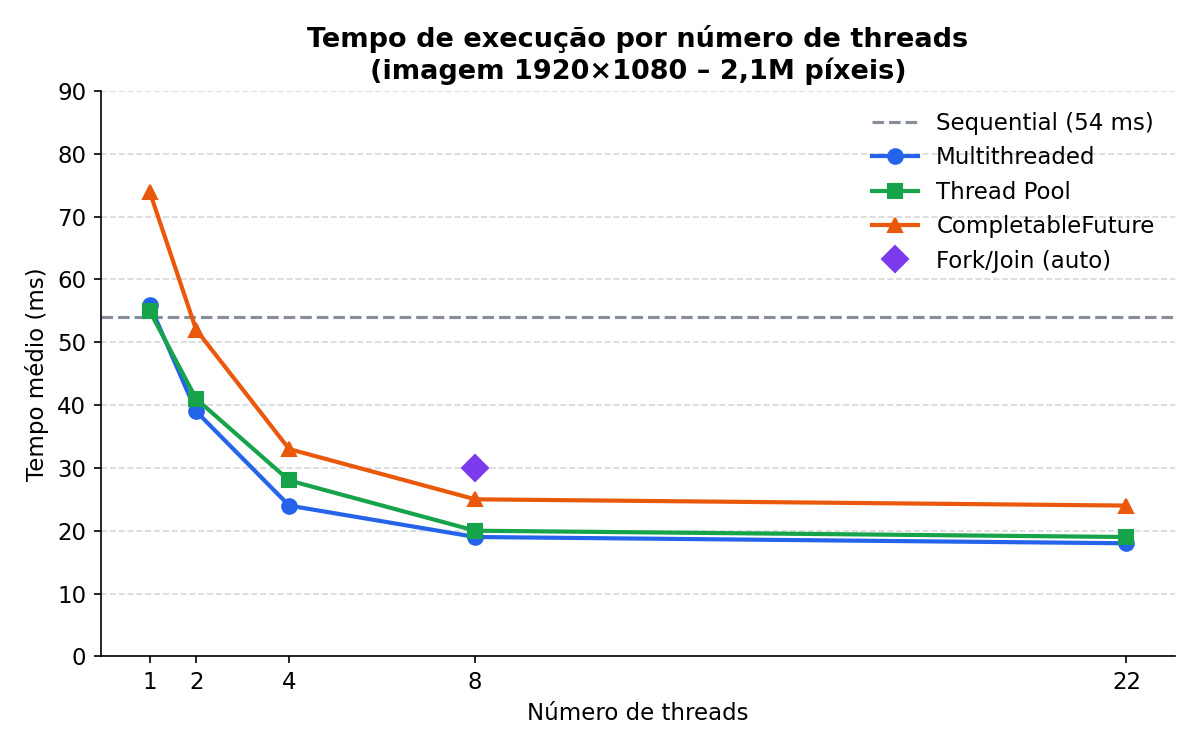
\includegraphics[width=0.85\textwidth]{../../images/charts/chart_06_time_threads_fhd.png}
    \caption{Tempo de execução por número de threads (imagem 1920×1080)}
    \label{fig:time_threads_fhd}
\end{figure}

O Fork/Join apresenta 30~ms nesta imagem, contra 18~ms do Multithreaded manual. Com 1080 linhas e \texttt{THRESHOLD=32}, o framework cria $\lceil 1080/32 \rceil = 34$ tarefas-folha, sobrecarregando o \textit{work-stealing scheduler} para uma granularidade que não justifica a divisão recursiva.

% ─────────────────────────────────────────────────────────────
\section{Overhead de Abstração e Memória}
% ─────────────────────────────────────────────────────────────

O CompletableFuture com 1 thread é consistentemente mais lento do que o Sequential em imagens grandes: 74~ms vs. 54~ms em Full~HD ($-$37\%), e 246~ms vs. 216~ms em 4K ($-$14\%). O overhead de \texttt{supplyAsync}, \texttt{allOf} e \texttt{thenApply} não é desprezável quando o trabalho útil por tarefa é pequeno.

O consumo de memória mantém-se estável entre implementações (~38--42~MB para a imagem 860×1276, ~76~MB para Full~HD, ~301~MB para 4K), refletindo maioritariamente o tamanho da imagem. O Multithreaded a 22T apresenta ~54~MB na imagem 860×1276 (+34\% face ao Sequential) devido à criação de 22 arrays \texttt{int[256]} de histograma parcial --- overhead de apenas ~22 KB, mas que fica visível na medição por diferença de heap.

% ─────────────────────────────────────────────────────────────
\section{Bottlenecks Identificados}
% ─────────────────────────────────────────────────────────────

\begin{enumerate}
    \item \textbf{Barreira sequencial (fase 2):} O histograma cumulativo (O(256)) é intrínsecamente sequencial e separa a fase 1 da fase 3, impedindo um pipeline contínuo.
    \item \textbf{Saturação de memória em 4K:} A 8.3M píxeis e 22 threads, adicionar mais cores não reduz o tempo --- todos os threads disputam o mesmo barramento de memória.
    \item \textbf{Criação de objetos \texttt{Color}:} A fase 3 instancia um \texttt{Color} por píxel (até 8.3M objetos por execução), pressionando o GC de forma independente do grau de paralelismo. Substituir por arrays \texttt{int[]} reduziria este custo.
\end{enumerate}

% ============================================================
\chapter{Conclusões}
% ============================================================

\section{Síntese dos Resultados}

Este projeto demonstrou que a paralelização da equalização de histograma produz ganhos reais, mas limitados pela estrutura do algoritmo e pelos recursos de hardware. Os resultados principais são:

\begin{itemize}
    \item O melhor speedup absoluto foi de \textbf{5.50×} (Multithreaded 8T e CompletableFuture 22T na imagem 860×1276, 33~ms~→~6~ms) numa máquina de 22 processadores.
    \item O \textbf{sweet spot} da paralelização situa-se em imagens de ~1M píxeis: grande o suficiente para amortizar o overhead de threading, pequeno o suficiente para caber em cache.
    \item Em imagens 4K (8.3M px), todas as implementações a 22T convergem para ~79--82~ms, limitadas pela \textbf{largura de banda de memória}, não pela capacidade de processamento.
    \item O \textbf{CompletableFuture com 1 thread é mais lento que o Sequential} em imagens grandes (overhead de 14--37\%), ilustrando que abstrações assíncronas têm custo real quando o trabalho por tarefa é pequeno.
    \item O \textbf{Fork/Join degrada em Full~HD} (30~ms vs. 18~ms Multithreaded): o THRESHOLD=32 linhas cria granularidade excessiva para 1080 linhas, sobrecarregando o work-stealing scheduler.
\end{itemize}

\section{Comparação das Implementações}

\begin{table}[H]
    \centering
    \caption{Comparação qualitativa das implementações}
    \label{tab:qualitative}
    \begin{tabular}{lllll}
        \toprule
        \textbf{Implementação} & \textbf{Throughput} & \textbf{Escalabilidade} & \textbf{Complexidade} & \textbf{Overhead} \\
        \midrule
        Sequential       & Baseline  & N/A         & Muito baixa & Nenhum \\
        Multithreaded    & Alto      & Boa até 8T  & Média       & Baixo \\
        Thread Pool      & Alto      & Boa até 22T & Média       & Baixo \\
        Fork/Join        & Médio-alto & Variável   & Alta        & Médio \\
        CompletableFuture & Alto     & Boa até 22T & Média       & Médio-alto (1T) \\
        \bottomrule
    \end{tabular}
\end{table}

\section{Garbage Collector}

O resultado mais surpreendente foi que o \textbf{Serial GC produz o melhor throughput} para este workload (43~ms sequential, 8~ms melhor paralelo), apesar de ter as pausas individuais mais longas. A causa é que o overhead do GC que afeta o tempo \emph{medido} é diferente das pausas STW: write barriers, threads de fundo concorrentes e overhead de alocação --- o Serial GC minimiza todos estes durante a execução da aplicação.

O \textbf{ZGC} é o pior para workloads compute-heavy de curta duração: os seus threads de marcação concorrentes disputam os 22 núcleos com a aplicação, penalizando +65\% o tempo sequencial.

O \textbf{G1GC} é adotado como configuração de referência por ser o padrão do JDK moderno e oferecer pausas previsíveis adequadas para uso interativo.

\section{Reflexão e Otimizações Futuras}

A \textbf{Lei de Amdahl} explica o comportamento observado: a fase do histograma cumulativo (O(256)) é intrínsecamente sequencial e constitui o teto teórico do speedup. Com uma fração sequencial estimada de ~5\%, o speedup máximo teórico seria ~15×; o valor obtido de 5.5× indica que overhead adicional (coordenação, memória, GC) reduz o speedup real para ~37\% do teórico.

Otimizações que aumentariam o speedup:
\begin{enumerate}
    \item \textbf{Substituir \texttt{Color[][]} por \texttt{int[][]}:} elimina 8.3M alocações de objeto por execução em 4K, reduzindo drasticamente a pressão no GC.
    \item \textbf{Ajustar o THRESHOLD do Fork/Join} por imagem --- um THRESHOLD dinâmico baseado em \texttt{rows / (2 * cores)} daria granularidade óptima independentemente da dimensão.
    \item \textbf{Processamento por blocos (tiling):} melhorar a localidade de cache processando blocos 2D em vez de fatias de linhas, especialmente benéfico em imagens largas.
\end{enumerate}

% ============================================================
\bibliographystyle{ACM-Reference-Format}
\renewcommand\bibname{Referências}

\begin{thebibliography}{9}

\bibitem{gonzalez2018}
R.C. Gonzalez and R.E. Woods.
\newblock \textit{Digital Image Processing}, 4th edition.
\newblock Pearson, 2018.

\bibitem{sedgewick2016}
Robert Sedgewick and Kevin Wayne.
\newblock \textit{Computer Science: An Interdisciplinary Approach}, 1st edition.
\newblock Addison-Wesley Professional, 2016.

\bibitem{goetz2006}
Brian Goetz et al.
\newblock \textit{Java Concurrency in Practice}.
\newblock Addison-Wesley, 2006.

\bibitem{oracle_forkjoin}
Oracle Corporation.
\newblock \textit{Fork/Join Framework}.
\newblock Java Documentation, 2024.
\newblock \url{https://docs.oracle.com/javase/tutorial/essential/concurrency/forkjoin.html}

\bibitem{oracle_completable}
Oracle Corporation.
\newblock \textit{CompletableFuture API}.
\newblock Java SE 21 Documentation, 2024.
\newblock \url{https://docs.oracle.com/en/java/javase/21/docs/api/java.base/java/util/concurrent/CompletableFuture.html}

\end{thebibliography}

\label{references}
\addcontentsline{toc}{chapter}{Referências}

\end{document}
